\documentclass[a4paper]{scrartcl}
\usepackage[utf8]{inputenc}
\usepackage[english]{babel}
\usepackage{graphicx}
\usepackage{lastpage}
\usepackage{pgf}
\usepackage{wrapfig}
\usepackage{fancyvrb}
\usepackage{fancyhdr}
\pagestyle{fancy}

\usepackage[colorlinks=true,linkcolor=violet]{hyperref}
\usepackage[figure]{hypcap} %jump to img instead of caption text

\def\code#1{\texttt{#1}}


% Create header and footer
\headheight 27pt
\pagestyle{fancyplain}
\lhead{\footnotesize{Network Programming, ID1212}}
\chead{\footnotesize{Homework 4: Currency Converter}}
\rhead{}
\lfoot{}
\cfoot{\thepage\ (\pageref{LastPage})}
\rfoot{}

% Create title page
\title{Homework 4: Currency Converter}
\subtitle{Network Programming, ID1212}
\author{Max Körlinge, korlinge@kth.se}
\date{3 December 2018}

\begin{document}

\maketitle


\section{Introduction}

\noindent This assignment was to develop a three-tier web application using web frameworks for all layers. The requested application was a web site where you can convert at least four currencies, optionally together with an admin interface to change current exchange rates. The requirements on the program were:

\begin{itemize}
    \item The program must be designed using a layered architecture and object-oriented design principles.
    \item The converter must be able to convert between at least 4 different currencies.
    \item The client must be a web browser.
    \item All layers in the server must programmed with the help of a framework. The videos connected to the assignment suggest Thymeleaf for the view, Spring for the controller, and Spring/JPA for model and integration layers.
    \item The server must handle transactions.
    \item Conversion rates must be stored in a database.
    \item The user interface must be informative, so the user knows what is going on.
\end{itemize}

The optional task was:

\begin{itemize}
    \item Create an admin interface for the application, where an admin can enter conversion rates between different currencies, and show the total number of currency conversions made by all users together since the application started. Conversion rates and the counter must be stored in the database.
\end{itemize}

The program was written in full by the author of this report, and both the basic and the optional tasks were completed.

\section{Literature Study}

To prepare for this assignment, all video material provided by the course on RMI and database access was viewed together with the code of the sample programs. Important information was gathered on how to communicate in a distributed java program using RMI, and how to access the database using JDBC and JPA, and the advantages of each.

\section{Method}

\noindent The program was written in Java using the IntelliJ IDE. Maven was used to handle dependencies. MySQL was chosen as the DBMS. Otherwise, the suggested frameworks were used (Thymeleaf, Spring, and JPA).

The timeline was as follows: first, watch the related lectures; second, create a preliminary layered design with skeleton classes, including Spring annotations; third, write the configuration files (\code{application.yml}, \code{pom.xml}, \code{@Config}, etc.) and see that the server program can start without error messages; fourth, create sample HTML documents and a Spring controller to see that Thymeleaf is hooked up and ready to go; fifth, create one logical method call that goes from the view all the way to the bottom of the stack (in this case, the call to show all available currencies); sixth, implement all other functionality required. 

\section{Result}

\noindent The complete source code can be found at \href{https://github.com/fongie/CurrencyConverter}{https://github.com/fongie/CurrencyConverter}.

\begin{itemize}
    \item The program had to be designed using object-oriented design principles. Since Spring tends to steer towards domain-driven design, a version of this was used for the layered architecture, similar to the sample program in the course, with slightly different names. The \code{presentation} layer holds the Spring controllers as well as data holding objects that originate from the view. When it needs logic from the rest of the program, it passes it to a so-called service in the \code{services} layer. This layer can make computations like calculating the conversions, and it also passes on necessery calls to the database. Database logic is handled in the \code{repositories} layer, where Spring repository interfaces are used to handle database calls. Lastly, data from the database is represented in the \code{data} layer, where JPA entities and their read-only DTO versions are located.

        Speaking of read-only DTO versions of entities, they are a way to maintain solid encapsulation in the program, as well as in general letting all classes keep as small a public interface as possible. High cohesion is maintained by the classes holding to their specific purpose, for example, there are separate controllers and service classes for each page of the application (the admin and the conversion page). This separation also helps to reduce coupling, there is for example no MVC-like controller that often has dependencies all over the place.

    \item The converter had to convert between at least four currencies, and it does. The currencies implemented in the development database are SEK, USD, EUR and GBP, but since all calls to list available currencies and their rates are dynamic and loaded from the database, one could include as many currencies as one would wish by simply adding a few rows to the database. Since it was not a requirement to be able to enter new currencies in the admin interface, such database calls to include more currencies would have to be manual though.
    \item 
    \item 
    \item 
    \item 
    \item 
\end{itemize}

\begin{figure}[h!]
    \begin{center}
        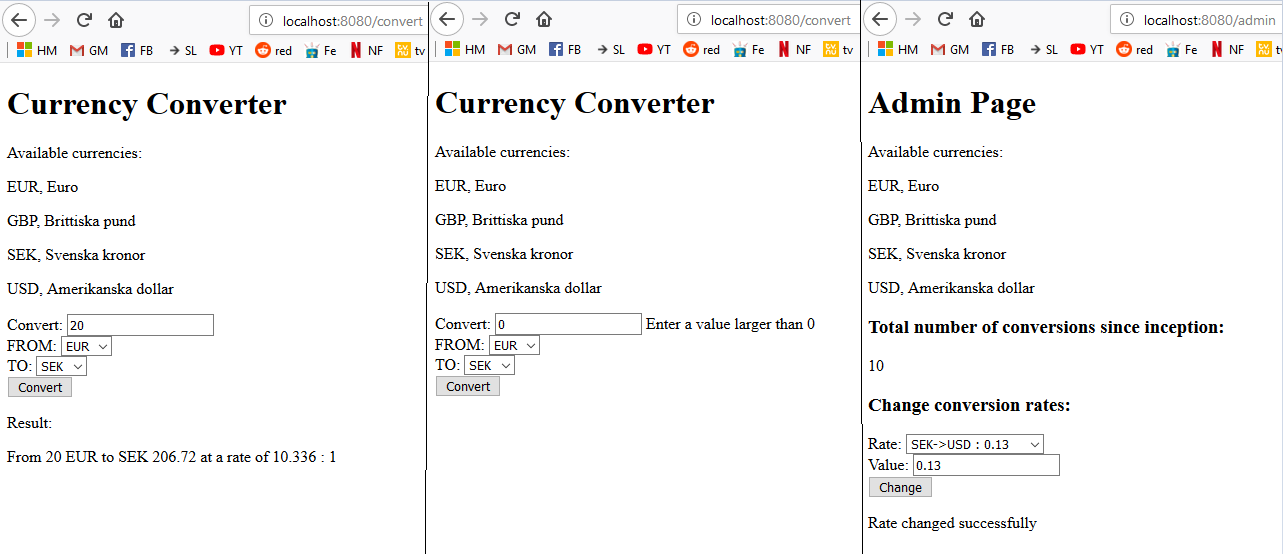
\includegraphics[scale=0.52]{ui.png}
        \caption{A sample output of the user interface}
        \label{fig:ui}
    \end{center}
\end{figure}



\section{Discussion}

This assignment was to develop a distributed application using RMI. The application was a file server, where a client can connect to and perform file operations on a remote catalog. Requirements concerned using RMI, using a database on the server side, not storing state on the client, having an informative user interface on the client, and structuring the program using object oriented design principles. All requirements were met and all functionality implemented. There was an optional task to send file contents using sockets, but this was not implemented due to time restraints.

Since I have not used RMI before, it was a learning experience and it took some time to get it to work the way I wanted it to. I have worked with databases in java before, so the JPA part was not very difficult.

The program could be improved mainly by implementing the optional task as well, which should not be too difficult, but circumstances have made it so that time right now is limited. You could also have a nice graphical interface to go with the program as well.


\section{Comments About the Course}

This was the most time consuming assignment so far, with a lot of lecture material and different integrating parts to work out. It unfortunately for me coincided with a big assignment in another course (Operating systems), and me working abroad during the weekends, so although I want to do the optional task because it is interesting and this assignment was very instructive, I can not do so in time.

I appreciate the way the course is structured, with large-ish practical programming tasks and no unnecessary time spent travelling to/from school due to recorded lectures, one of the best ways to learn in my opinion.

I spent quite a lot of time on this assignment but spread out over several days during some period of time, so it is difficult to pinpoint the exact hours. Probably around 5 hours on lecture material, 15-20 hours on the code and 3 hours on the report.

\end{document}
